%UNIT 13: SECOND ORDER LINEAR DEs
%%%%%%%%%%%%%%%%%%%%%%%%%%%
%%%% Put the following at the top of each .tex file  %
\pagestyle{fancy}
\renewcommand{\theUnit}{2.5}
\ifthenelse{\isundefined{\UnitPageNumbers}}{}{\setcounter{page}{1}}
\rhead{Section \theUnit: Nonhomogeneous Equations}
\lhead{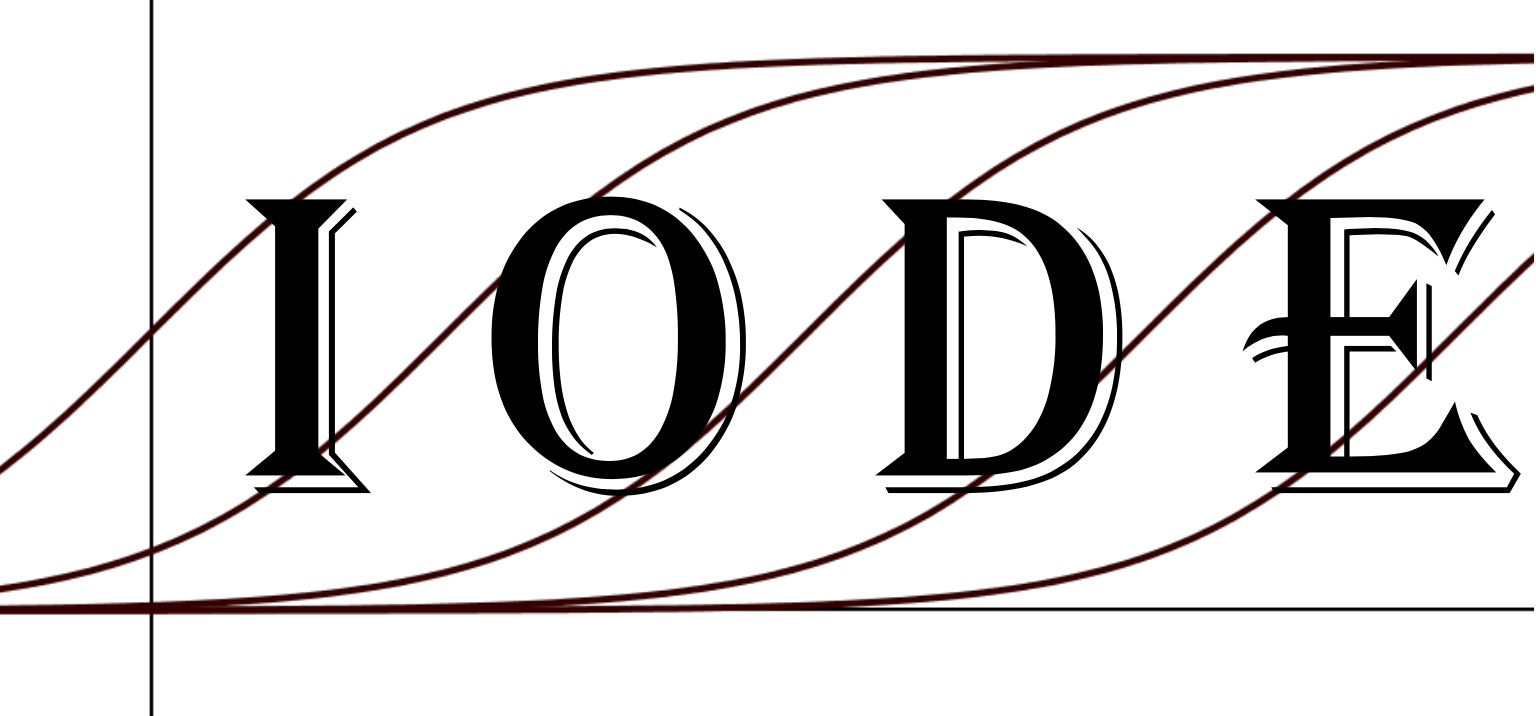
\includegraphics[width=1.25cm]{IODE-logo.png}}
\rfoot{\mypage}
\lfoot{}
\cfoot{}
\fancypagestyle{firstfooter}{\footskip = 50pt}
\renewcommand{\footrulewidth}{.4pt}
%%%%%%%%%%%%%%%%%%%%%%%%%%%
\vspace*{-20pt} \thispagestyle{firstfooter}
\pagebegin{Guess and Test for Nonhomogeneous Cases}

So far we have been using patterns recognized in wisely guessing the form of solutions to homogeneous second order differential equations of the form $ay''+by'+cy = 0$.  Can we adjust our guesses to handle nonhomogeneous differential equations as well?

\begin{enumerate}
\item Find a solution to the following \textbf{nonhomogeneous} differential equation:
\[
\frac{d^2x}{dt^2}+10\frac{dx}{dt}+9x=18.
\]
What is your best guess for a function whose second derivative plus 10 times its first derivative plus 9 times the function itself sum to 18? Test out your guess to see if it works. If it doesn't work keep trying. \label{13problem8}

\vfill
\end{enumerate}

The solution you found in the previous problem is called the \textbf{particular solution} to the nonhomogeneous differential equation it is not the general solution. For now we will focus on how we can find the particular solution by wisely guessing their general form based on the nonhomogeneous part of the differential equation. We will soon combine what we know about the homogeneous case and particular solutions to find general solutions. %To find the general solution to the nonhomogeneous differential equation you simply add the particular solution to the general solution to the corresponding homogeneous equation. This 3-step strategy (1 - Find the general solution to the corresponding homogeneous equation; 2 - Find the particular solution to the nonhomogeneous equation, 3 - Add the previous results) is called the \textbf{Method of Undetermined Coefficients}.

\clearpage

\begin{enumerate}[resume]
\item Find a solution to the following nonhomogeneous differential equation:
\[
\frac{d^2x}{dt^2}+10\frac{dx}{dt}+9x=18t.
\]
What is your best guess? Test out your guess to see if it works. If it doesn't work keep trying. \label{13problem8}
\vfill

\ii Based on the previous examples, what would be a good guess for the general form of the particular solution to
\[
\frac{d^2x}{dt^2}+10\frac{dx}{dt}+9x=18t^3.
\]
Your guess should have depend on constants whose values you do not need to determine for this example.
\vspace{1in}

\clearpage

\item Sean and Phil are trying to find the particular solution to $\displaystyle\frac{d^2x}{dt^2}+10\frac{dx}{dt}+9x=85\sin(2t)$. Sean guesses $x(t)=A\sin(2t)$ for the particular solution and Phil guesses $x(t)=B\cos(2t)$. \label{13problem10}

\begin{enumerate}
\item Do you think these are reasonable guesses? Explain why or why not. \label{13problem10parta} \vspace{2in}
\item For each of their guesses, can you find a value of $A$ or $B$ such that their guess is a solution? If yes, write down the general solution. If no, come up with a different guess for the particular solution and show that your guess is correct. \label{13problem10partb} \vfill
\end{enumerate}

\clearpage

\item Consider the nonhomogeneous differential equation \label{13problem15parta}
\[
\frac{d^2x}{dt^2}+25x=10\cos(5t)
\]
\bb
\ii Suppose you wish to find the particular solution to this differential equation. Explain why a guess of the form $x(t) = A\cos(5t) + B\sin(5t)$ is doomed to fail. \vspace{1in}
\item Nevertheless, explain why your particular solution must have terms that \textit{look like} $\cos(5t)$ and $\sin(5t)$. \label{13problem15partb} \vspace{1in}
\item For an unknown differentiable function $f(t)$, write down the first and second derivatives of $tf(t)$, what do you notice? \label{13problem15partc} \vspace{1in}
\item Explain why a guess of $At\cos(5t)$ is insufficient to find the particular solution. \label{13problem15partd} \vspace{1in}

\item Use the guess $x(t) = t(A\cos(5t) + B\sin(5t))$ to find a particular solution to the above equation. \label{13problem15parte} \vfill

\end{enumerate}
\end{enumerate}

\clearpage

The previous exercise is an example of \textbf{resonance}, which occurs when an external force has the same properties (such as frequency) as the general homogeneous solution. Practically speaking, when the homogeneous and nonhomogeneous parts of the differential equation have resonance this creates a huge increase in energy (that may even cause a bridge to collapse). 


\begin{enumerate}[resume]
\ii For each of the examples circle the word(s) that correctly describe whether the nonhomogeneous differential equation has resonance or not.

\bb
\ii $x''+25x=10\cos(5t)$ (\ \ \ does\ \ \  or \ \ \ does not \ \ \ ) have resonance since $x_H = C_1\cos{(5t)}+ C_2 \sin{(5t)}$.\bs
\ii $x''+25x=10e^{5t}$  (\ \ \ does\ \ \  or \ \ \ does not \ \ \ ) resonance since $x_H = C_1\cos{(5t)}+ C_2 \sin{(5t)}$. \bs
\ii $x''-3x'-10x=10\cos(5t)$  (\ \ \ does\ \ \  or \ \ \ does not \ \ \ ) resonance since $x_H = C_1e^{5t}+ C_2 e^{-2t}$. \bs
\ii $x''-3x'-10x=10e^{5t}$  (\ \ \ does\ \ \  or \ \ \ does not \ \ \ ) resonance since $x_H = C_1e^{5t}+ C_2 e^{-2t}$. \bs
\ii $x''+2x'+ 17x=6e^{-t} \sin{(4t)} $  (\ \ \ does\ \ \  or \ \ \ does not \ \ \ ) resonance since $x_H = C_1e^{-t}\cos{(4t)}+ C_2 e^{-t}\sin{(4t)}$. \bs
\ii $x''+2x'+ 17x=6 \sin{(4t)} $  (\ \ \ does\ \ \  or \ \ \ does not \ \ \ ) resonance since $x_H = C_1e^{-t}\cos{(4t)}+ C_2 e^{-t}\sin{(4t)}$. \bs
\ee

Whenever resonance is present between the homogeneous solution and nonhomogeneous forcing function, we can adjust
our initial guess by multiplying by a factor of $t$. For example, since\newline $x''+25x=10\cos(5t)$ has resonance our guess for the particular solution is
\[ x_p = t \big(  A\cos{(5t)}+ B \sin{(5t)} \big).\]

\ii For each of the examples in the previous question where there was resonance, give the initial guess for the particular solution. Do not solve for the values of the undetermined coefficients.

\vfill

\clearpage


\ii What would be a good guess for the general form of the particular solution to
\[ \frac{d^2y}{dt^2}-6\frac{dy}{dt}+9y=5e^{3t} \mbox{?}\]
Do not find the values of the undetermined coefficients. \vfill

\ii What would be a good guess for the general form of the particular solution to
\[ \frac{d^2y}{dt^2}-6\frac{dy}{dt}+9y=5e^{3t}\cos{(2t)} \mbox{?}\]
Do not find the values of the undetermined coefficients.  \vfill

\ii What would be a good guess for the general form of the particular solution to
\[ \frac{d^2y}{dt^2}-6\frac{dy}{dt}+9y=5t^2e^{3t}\cos{(2t)} \mbox{?}\]
Do not find the values of the undetermined coefficients.  \vfill



\end{enumerate}



